\documentclass{article}
\usepackage[T1]{fontenc}
\usepackage{lmodern}
\usepackage{graphicx}
\usepackage{amsmath,amssymb}
\usepackage[a4paper,margin=2cm]{geometry}
\usepackage[absolute,overlay]{textpos}
\setlength{\TPHorizModule}{1mm}
\setlength{\TPVertModule}{1mm}
\usepackage[indonesian]{babel}
\usepackage{hyperref}
\setlength{\emergencystretch}{2em}
% unit: Halaman 22

\begin{document}

% === Halaman 22 (llm) ===

\begin{itemize}
    \item Demo Merkle-Hellman knapsack online:
    \url{https://asecuritysite.com/encryption/knapcode?val1=3%2C%205%2C%2015%2C%2025%2C%2054%2C%20110%2C%20225&val2=10&val3=439&val4=1001000110010110110011011111}
\end{itemize}

\vspace{10mm}

% deskripsi: Screenshot aplikasi web simulasi Knapsack Encryption (Merkle-Hellman Knapsack) yang menunjukkan input kunci privat, n, modulus, dan data, serta hasil perhitungan kunci publik, cipher, inverse, dan plaintext.
% bbox normalisasi: [0.0000, 0.2700, 1.0000, 0.9700]
\begin{textblock*}{210.00mm}(0.00mm,80.19mm)
\noindent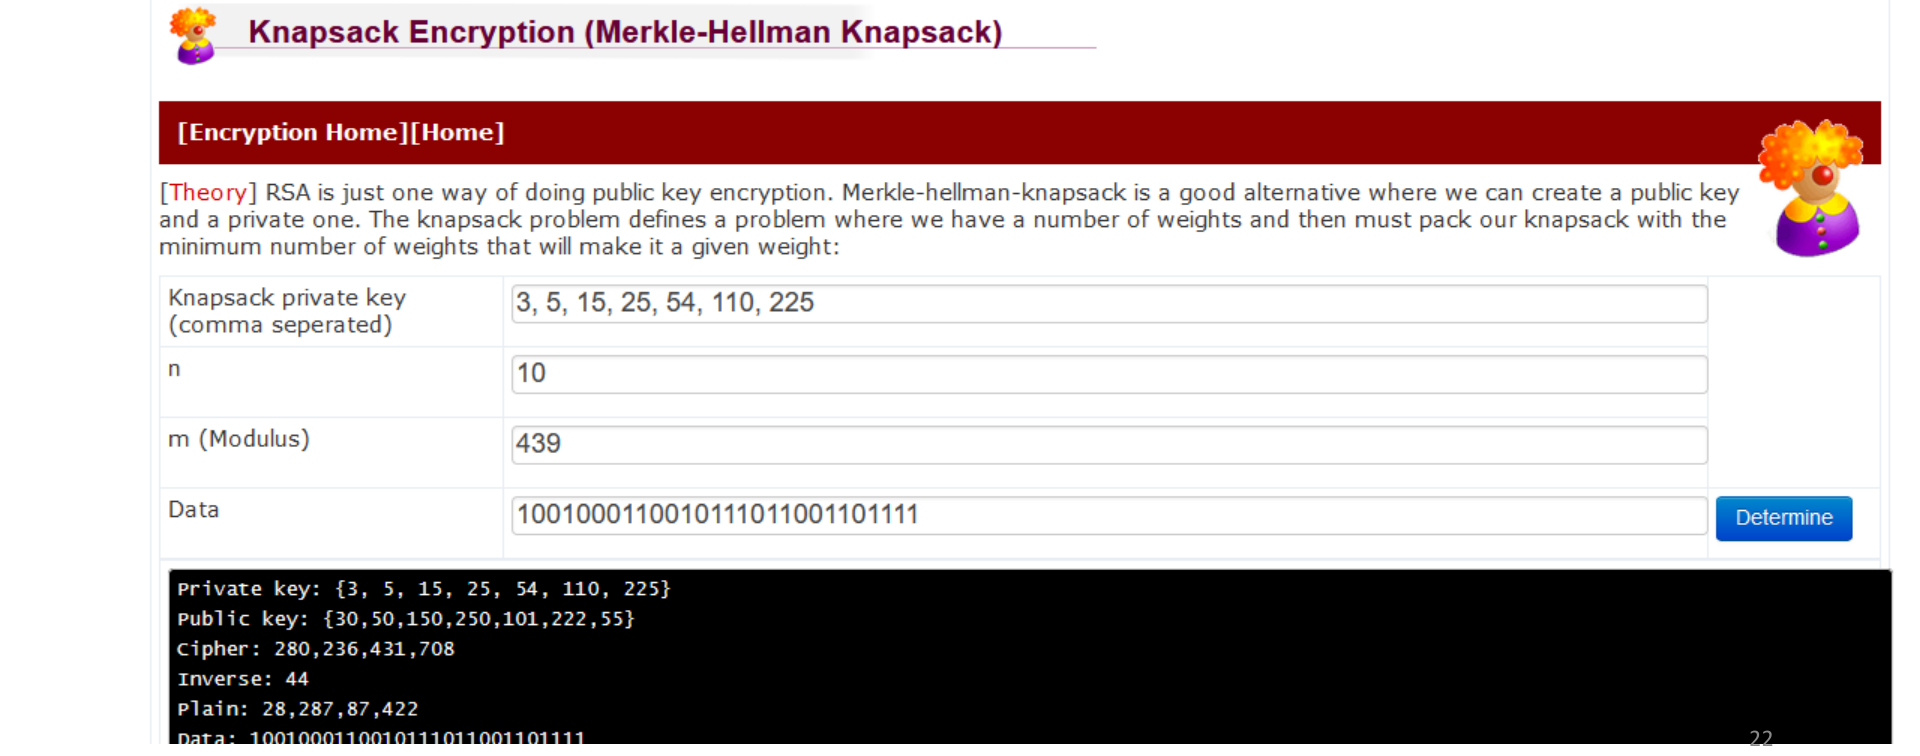
\includegraphics[width=210.00mm,height=207.90mm]{../../images/llm/page_022_img_01.png}%
\end{textblock*}

\end{document}
